\documentclass{article}

% content/resources/templates/preamble.tex
\usepackage[margin=0.6in]{geometry}
\author{Milav Dabgar}
\usepackage{amsmath,amssymb,amsthm}
\usepackage{booktabs}
\usepackage{multirow}
\usepackage{xcolor}
\usepackage{tcolorbox}
\tcbuselibrary{breakable,skins}
\usepackage[colorlinks=true,linkcolor=blue]{hyperref}
\usepackage{titlesec}
\usepackage{enumitem}
\usepackage{tikz}
\usepackage{pgfplots}
\usepackage{circuitikz}
\usepackage[version=4]{mhchem}
\usepackage{longtable}
\usepackage{array}
\usepackage{float}
\usepackage{caption}
\usepackage{listings}

\lstset{
  basicstyle=\small\ttfamily,
  breaklines=true,
  breakatwhitespace=false,
  postbreak=\mbox{\textcolor{red}{$\hookrightarrow$}\space},
  float=false,
  numbers=left,
  numberstyle=\tiny\color{gray},
  numbersep=10pt,
  xleftmargin=2em,
  keywordstyle=\color{blue},
  commentstyle=\color{green!60!black},
  stringstyle=\color{purple},
  backgroundcolor=\color{gray!5},
  showstringspaces=false,
  tabsize=2,
  captionpos=b,
  keepspaces=true,
  columns=flexible
}

\pgfplotsset{compat=1.18}
\usetikzlibrary{shapes,arrows,positioning,calc,patterns,decorations.pathmorphing,decorations.markings,arrows.meta}

% Color scheme
\definecolor{headcolor}{RGB}{0,102,204}
\definecolor{keycolor}{RGB}{220,20,60}
\definecolor{solutioncolor}{RGB}{34,139,34}
\definecolor{mnemoniccolor}{RGB}{148,0,211}
\definecolor{codecolor}{RGB}{0,0,100}

% Spacing
\setlength{\parskip}{3pt}
\setlist[itemize]{nosep}
\setlist[enumerate]{nosep}

% Title formatting
\titleformat{\section}{\Large\bfseries\color{headcolor}}{\thesection}{1em}{}
\titleformat{\subsection}{\large\bfseries\color{headcolor}}{\thesubsection}{1em}{}

% Pandoc tightlist compatibility
\providecommand{\tightlist}{%
  \setlength{\itemsep}{0pt}\setlength{\parskip}{0pt}}

% Pandoc longtable compatibility
\newcounter{none}
\def\thenone{}


% content/resources/templates/english-boxes.tex

% Custom environments
\newtcolorbox{solutionbox}{
 breakable,
 enhanced,
 colback=solutioncolor!5!white,
 colframe=solutioncolor!75!black,
 fonttitle=\bfseries,
 title=Solution
}

\newtcolorbox{solutionboxnobreak}{
 colback=solutioncolor!5!white,
 colframe=solutioncolor!75!black,
 fonttitle=\bfseries,
 title=Solution
}

\newtcolorbox{keyformula}{
 breakable,
 enhanced,
 colback=keycolor!5!white,
 colframe=keycolor!75!black,
 fonttitle=\bfseries,
 title=Key Formula
}

\newtcolorbox{mnemonicboxenv}{
 breakable,
 enhanced,
 colback=mnemoniccolor!5!white,
 colframe=mnemoniccolor!75!black,
 fonttitle=\bfseries,
 title=Mnemonic
}

\newcommand{\mnemonicbox}[1]{%
  \begin{mnemonicboxenv}
    #1
  \end{mnemonicboxenv}
}


% Custom commands for GTU solutions
% This file defines semantic commands for consistent formatting

% Question command with automatic formatting
\newcommand{\question}[2]{%
  \section*{Question #1}%
  \textbf{#2}%
}

% OR question variant
\newcommand{\questionor}[2]{%
  \section*{Question #1 OR}%
  \textbf{#2}%
}

% Proper table environment with caption
\newenvironment{answertable}[1]{%
  \begin{table}[htbp]
  \centering
  \caption{#1}
}{%
  \end{table}
}

% Proper figure environment for diagrams
\newenvironment{answerdiagram}[1]{%
  \begin{figure}[htbp]
  \centering
  \caption{#1}
}{%
  \end{figure}
}

% Semantic markup for key terms
\newcommand{\keyword}[1]{\textbf{#1}}
\newcommand{\code}[1]{\texttt{#1}}
\newcommand{\classname}[1]{\texttt{#1}}
\newcommand{\methodname}[1]{\texttt{#1}}

% Proper quotation marks
\newcommand{\mnemonic}[1]{``#1''}


\title{Principles of Electronic Communication (4331104) - Winter 2024 Solution}
\date{December 09, 2024}

\begin{document}
\maketitle

\questionmarks{1}{a}{3}
\textbf{What is modulation? What is the need of it?}

\begin{solutionbox}
    \textbf{Modulation} is the process of varying one or more properties (amplitude, frequency, or phase) of a high-frequency carrier signal according to the instantaneous value of a lower frequency message signal.

    \textbf{Need for modulation:}
    \begin{itemize}
        \item \textbf{Antenna size reduction}: Allows practical antenna size ($\lambda/4$).
        \item \textbf{Multiplexing}: Enables multiple signals to share same medium.
        \item \textbf{Interference reduction}: Shifts signal to suitable frequency band.
        \item \textbf{Range extension}: Increases transmission distance.
    \end{itemize}

    \begin{mnemonicbox}
    "AMIR" - Antenna, Multiplexing, Interference, Range
    \end{mnemonicbox}
\end{solutionbox}

\questionmarks{1}{b}{4}
\textbf{Derive the expression for DSBFC of AM wave.}

\begin{solutionbox}
    DSBFC (Double Sideband Full Carrier) AM wave derivation:

    \textbf{Mathematical derivation:}
    \begin{itemize}
        \item Carrier signal: $c(t) = A_c \cos(\omega_c t)$
        \item Message signal: $m(t) = A_m \cos(\omega_m t)$
        \item AM signal: $s(t) = A_c[1 + \mu m(t)]\cos(\omega_c t)$
        \item Where $\mu = \text{modulation index} = A_m/A_c$
    \end{itemize}

    \textbf{Substituting message signal:}
    \begin{align*}
        s(t) &= A_c[1 + \mu \cos(\omega_m t)]\cos(\omega_c t) \\
        s(t) &= A_c \cos(\omega_c t) + \mu A_c \cos(\omega_m t)\cos(\omega_c t)
    \end{align*}

    \textbf{Using trigonometric identity:}
    \[ \cos(A)\cos(B) = \frac{1}{2}[\cos(A+B) + \cos(A-B)] \]

    \textbf{Final expression:}
    \[ s(t) = A_c \cos(\omega_c t) + \frac{\mu A_c}{2}[\cos((\omega_c+\omega_m)t) + \cos((\omega_c-\omega_m)t)] \]

    \begin{center}
    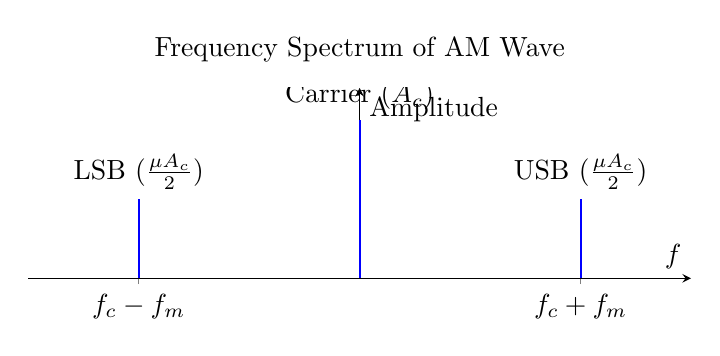
\begin{tikzpicture}
        \begin{axis}[
            width=10cm, height=4cm,
            axis lines=middle,
            xtick={-1, 0, 1}, xticklabels={$f_c-f_m$, $f_c$, $f_c+f_m$},
            ytick={\empty},
            ymin=0, ymax=1.2,
            xmin=-1.5, xmax=1.5,
            xlabel={$f$}, ylabel={Amplitude},
            title={Frequency Spectrum of AM Wave}
        ]
            \addplot[ycomb, mark=none, thick, blue] coordinates {
                (0, 1) (-1, 0.5) (1, 0.5)
            };
            \node[above] at (axis cs:0,1) {Carrier ($A_c$)};
            \node[above] at (axis cs:-1,0.5) {LSB ($\frac{\mu A_c}{2}$)};
            \node[above] at (axis cs:1,0.5) {USB ($\frac{\mu A_c}{2}$)};
        \end{axis}
    \end{tikzpicture}
    \captionof{figure}{Spectrum of DSBFC AM Wave}
    \end{center}
\end{solutionbox}

\questionmarks{1}{c}{7}
\textbf{Classify Noise signal and explain flicker noise, shot noise and thermal noise.}

\begin{solutionbox}
    \textbf{Noise Classification:}

    \begin{center}
    \begin{tabulary}{\linewidth}{L L L}
        \hline
        \textbf{Type} & \textbf{Source} & \textbf{Characteristics} \\
        \hline
        \textbf{External Noise} & Environmental sources & Outside communication system \\
        \textbf{Internal Noise} & Components & Generated within system \\
        \hline
    \end{tabulary}
    \captionof{table}{Types of Noise}
    \end{center}

    \textbf{Types of internal noise:}

    \begin{enumerate}
        \item \textbf{Flicker Noise:}
        \begin{itemize}
            \item \textbf{Source}: Occurs in active devices.
            \item \textbf{Characteristics}: Inversely proportional to frequency ($1/f$).
            \item \textbf{Effect}: Dominant at low frequencies.
        \end{itemize}

        \item \textbf{Shot Noise:}
        \begin{itemize}
            \item \textbf{Source}: Random electron flow across junctions.
            \item \textbf{Characteristics}: Independent of frequency (white noise).
            \item \textbf{Effect}: Random current fluctuations in diodes/transistors.
        \end{itemize}

        \item \textbf{Thermal Noise:}
        \begin{itemize}
            \item \textbf{Source}: Random motion of electrons due to temperature.
            \item \textbf{Characteristics}: Present in all conductors, resistors.
            \item \textbf{Formula}: $P_n = kTB$ ($k=\text{Boltzmann constant}$, $T=\text{temperature}$, $B=\text{bandwidth}$).
            \item \textbf{Effect}: Sets noise floor in receivers.
        \end{itemize}
    \end{enumerate}

    \begin{mnemonicbox}
    "FST" - Flicker decreases with Frequency, Shot is from electron flow, Thermal depends on Temperature
    \end{mnemonicbox}
\end{solutionbox}

\questionmarks{1}{c}{7}
\textbf{Describe EM wave also write at least one application of different band of spectrum.}

\begin{solutionbox}
    \textbf{EM Wave:}
    Electromagnetic waves are energy propagating through space as time-varying electric and magnetic fields, traveling at speed of light ($3\times10^8$ m/s).

    \textbf{Characteristics:}
    \begin{itemize}
        \item Transverse waves with E and H fields perpendicular to each other.
        \item No medium required for propagation.
        \item Described by wavelength ($\lambda$) and frequency ($f$).
        \item Relation: $c = f \times \lambda$.
    \end{itemize}

    \textbf{EM Spectrum and Applications:}

    \begin{center}
    \begin{tabulary}{\linewidth}{L L L}
        \hline
        \textbf{Frequency Band} & \textbf{Frequency Range} & \textbf{Application} \\
        \hline
        ELF & 3Hz-30Hz & Submarine communication \\
        VLF & 3kHz-30kHz & Navigation systems \\
        LF & 30kHz-300kHz & AM broadcasting \\
        MF & 300kHz-3MHz & AM radio broadcasting \\
        HF & 3MHz-30MHz & Shortwave radio \\
        VHF & 30MHz-300MHz & FM radio, TV broadcasting \\
        UHF & 300MHz-3GHz & TV, mobile phones, WiFi \\
        SHF & 3GHz-30GHz & Satellite communication, radar \\
        EHF & 30GHz-300GHz & Millimeter wave communication \\
        Infrared & 300GHz-400THz & Remote controls, thermal imaging \\
        Visible & 400THz-800THz & Fiber optic communication \\
        Ultraviolet & 800THz-30PHz & Sterilization, authentication \\
        X-Rays & 30PHz-30EHz & Medical imaging \\
        Gamma Rays & >30EHz & Cancer treatment \\
        \hline
    \end{tabulary}
    \captionof{table}{EM Spectrum and Applications}
    \end{center}

    \begin{center}
    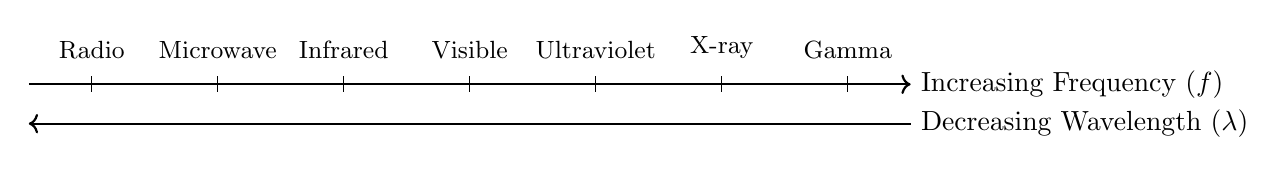
\begin{tikzpicture}[xscale=0.8]
        \draw[->, thick] (0,0) -- (14,0) node[right] {Increasing Frequency ($f$)};
        \draw[<-, thick] (0,-0.5) -- (14,-0.5) node[right] {Decreasing Wavelength ($\lambda$)};

        \foreach \x/\label in {1/Radio, 3/Microwave, 5/Infrared, 7/Visible, 9/Ultraviolet, 11/X-ray, 13/Gamma} {
            \draw (\x,0.1) -- (\x,-0.1);
            \node[above, align=center, font=\small] at (\x,0.2) {\label};
        }
    \end{tikzpicture}
    \captionof{figure}{Electromagnetic Spectrum}
    \end{center}

    \begin{mnemonicbox}
    "RMIUXG" - Radio, Microwave, Infrared, Ultraviolet, X-ray, Gamma
    \end{mnemonicbox}
\end{solutionbox}

\questionmarks{2}{a}{3}
\textbf{State advantages of SSB over DSB.}

\begin{solutionbox}
    \textbf{Advantages of SSB over DSB:}

    \begin{center}
    \begin{tabulary}{\linewidth}{L L}
        \hline
        \textbf{Parameter} & \textbf{SSB Advantage} \\
        \hline
        \textbf{Bandwidth} & 50\% less bandwidth requirement \\
        \textbf{Power} & Power saving of 33-83\% over AM/DSB \\
        \textbf{Transmitter} & Less power amplification needed \\
        \textbf{Receiver} & Simpler design without phase distortion \\
        \textbf{SNR} & Better signal-to-noise ratio \\
        \textbf{Fading} & Less susceptible to selective fading \\
        \hline
    \end{tabulary}
    \end{center}

    \begin{mnemonicbox}
    "BP TRFS" - Bandwidth, Power, Transmitter, Receiver, Fading, SNR
    \end{mnemonicbox}
\end{solutionbox}

\questionmarks{2}{b}{4}
\textbf{Explain generation of FM wave using FET reactance modulator.}

\begin{solutionbox}
    \textbf{FET Reactance Modulator:}

    \textbf{Working principle:}
    \begin{itemize}
        \item Uses FET as voltage-controlled reactance.
        \item Changes effective capacitance based on modulating signal.
        \item Connected across LC tank circuit of oscillator.
    \end{itemize}

    \textbf{Circuit operation:}
    \begin{enumerate}
        \item Modulating signal applied to gate of FET.
        \item FET drain-source resistance varies with gate voltage.
        \item Capacitive reactance changes with modulating signal.
        \item Oscillator frequency deviates with input signal.
    \end{enumerate}

    \begin{center}
    \begin{circuitikz}[font=\footnotesize]
        % FET
        \node[nfet] (fet) at (0,0) {};
        \node[right] at (fet.S) {S};
        \node[right] at (fet.D) {D};
        \node[left] at (fet.G) {G};
        
        % Components around FET
        \draw (fet.D) -- ++(0,1) coordinate (top);
        \draw (fet.S) -- ++(0,-1) coordinate (bottom) node[ground]{};
        
        \draw (top) to[C, l=$C_1$] ++(-2,0) coordinate (topleft) -- ++(0,-1) coordinate (Gconnect);
        \draw (Gconnect) -- (fet.G);
        \draw (Gconnect) to[R, l=$R_1$] (Gconnect |- bottom) -- (bottom);
        
        \draw (topleft) -- ++(-1,0) node[circ]{} node[left]{To Tank Circuit};
        \draw (bottom -| topleft) -- ++(-1,0) node[circ]{} node[left]{Ground};
        
        % Input
        \draw (fet.G) -- ++(-0.5,0) to[C, l=$C_{in}$] ++(-1,0) node[left] {$V_{in}$ (Modulating)};
        
        % RFC
        \draw (top) to[L, l=RFC] ++(2,0) node[right] {$V_{DD}$};
        
    \end{circuitikz}
    \captionof{figure}{FET Reactance Modulator}
    \end{center}

    \textbf{Key features:}
    \begin{itemize}
        \item \textbf{Simple design}: Fewer components than other modulators.
        \item \textbf{Linearity}: Good for wide-band FM generation.
        \item \textbf{Stability}: Temperature stable compared to varactor diodes.
    \end{itemize}

    \begin{mnemonicbox}
    "LOVE FM" - LC Oscillator with Voltage-controlled Element for FM
    \end{mnemonicbox}
\end{solutionbox}

\questionmarks{2}{c}{7}
\textbf{Derive the equation for total power in AM, calculate percentage of power savings in DSB and SSB.}

\begin{solutionbox}
    \textbf{Power in AM signal:}
    
    For AM signal $s(t) = A_c[1 + \mu\cos(\omega_m t)]\cos(\omega_c t)$

    \textbf{Total power calculation:}
    \begin{enumerate}
        \item Power in carrier: $P_c = A_c^2/2$
        \item Power in sidebands: $P_s = \mu^2 A_c^2/4$ (total for both sidebands)
        \item Total power: $P_t = P_c + P_s = \frac{A_c^2}{2} (1 + \frac{\mu^2}{2})$
    \end{enumerate}

    \textbf{For 100\% modulation ($\mu=1$):}
    \begin{itemize}
        \item $P_t = P_c \times (1 + 0.5) = 1.5 \times P_c$
        \item Carrier power = 66.67\% of total
        \item Sideband power = 33.33\% of total
    \end{itemize}

    \textbf{Power savings:}
    \begin{enumerate}
        \item \textbf{In DSB-SC:} 
        \begin{itemize}
            \item Carrier is suppressed.
            \item Power saved = 66.67\%
        \end{itemize}

        \item \textbf{In SSB:}
        \begin{itemize}
            \item Carrier + one sideband suppressed.
            \item Power saved = 66.67\% + 16.67\% = 83.33\%
        \end{itemize}
    \end{enumerate}

    \textbf{Comparative Table:}
    \begin{center}
    \begin{tabulary}{\linewidth}{L L L L L}
        \hline
        \textbf{Modulation} & \textbf{Carrier Power} & \textbf{Sideband Power} & \textbf{Total Power} & \textbf{Power Saving} \\
        \hline
        AM ($\mu=1$) & 100\% & 50\% & 150\% & 0\% \\
        DSB-SC & 0\% & 50\% & 50\% & 66.67\% \\
        SSB & 0\% & 25\% & 25\% & 83.33\% \\
        \hline
    \end{tabulary}
    \end{center}

    \begin{mnemonicbox}
    "CST" - Carrier power, Sideband power, Total power
    \end{mnemonicbox}
\end{solutionbox}

\questionmarks{2}{a}{3}
\textbf{Draw and explain Time domain and Frequency domain display of AM wave.}

\begin{solutionbox}
    \textbf{Time Domain and Frequency Domain Display of AM Wave:}

    \textbf{Time Domain:}
    \begin{itemize}
        \item Shows amplitude variations over time.
        \item Envelope follows modulating signal.
        \item Maximum amplitude: $A_{max} = A_c(1+\mu)$
        \item Minimum amplitude: $A_{min} = A_c(1-\mu)$
        \item Modulation index: $\mu = (A_{max}-A_{min})/(A_{max}+A_{min})$
    \end{itemize}

    \textbf{Frequency Domain:}
    \begin{itemize}
        \item Shows power distribution across frequencies.
        \item Carrier at center frequency $f_c$.
        \item Upper sideband at $f_c+f_m$.
        \item Lower sideband at $f_c-f_m$.
        \item Bandwidth = $2f_m$.
    \end{itemize}

    \begin{center}
    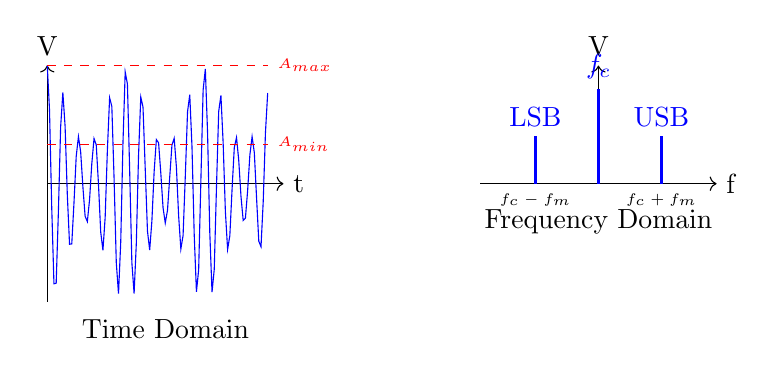
\begin{tikzpicture}
        % Time Domain
        \begin{scope}[xshift=-3.5cm]
            \draw[->] (0,-1.5) -- (0,1.5) node[above] {V};
            \draw[->] (0,0) -- (3,0) node[right] {t};
            \draw[blue, domain=0:2.8, samples=100] plot (\x, { (1 + 0.5*cos(deg(2*pi*\x))) * cos(deg(10*pi*\x)) });
            \node[below] at (1.5,-1.6) {Time Domain};
            \draw[red, dashed] (0,1.5) -- (2.8, 1.5) node[right, font=\tiny] {$A_{max}$};
             \draw[red, dashed] (0,0.5) -- (2.8, 0.5) node[right, font=\tiny] {$A_{min}$};
        \end{scope}

        % Frequency Domain
        \begin{scope}[xshift=3.5cm]
             \draw[->] (0,0) -- (0,1.5) node[above] {V};
            \draw[->] (-1.5,0) -- (1.5,0) node[right] {f};
            \draw[thick, blue] (0,0) -- (0,1.2) node[above] {$f_c$};
            \draw[thick, blue] (-0.8,0) -- (-0.8,0.6) node[above] {LSB};
            \draw[thick, blue] (0.8,0) -- (0.8,0.6) node[above] {USB};
            \node[below] at (0,-0.2) {Frequency Domain};
            \node[below, font=\tiny] at (-0.8,0) {$f_c-f_m$};
            \node[below, font=\tiny] at (0.8,0) {$f_c+f_m$};
        \end{scope}
    \end{tikzpicture}
    \captionof{figure}{AM Time and Frequency Domain Representations}
    \end{center}

    \begin{mnemonicbox}
    "TEF" - Time domain shows Envelope, Frequency domain shows spectral components
    \end{mnemonicbox}
\end{solutionbox}

\questionmarks{2}{b}{4}
\textbf{Explain pre-emphasis \& de-emphasis circuit.}

\begin{solutionbox}
    \textbf{Pre-emphasis and De-emphasis Circuits:}

    \textbf{Purpose:}
    \begin{itemize}
        \item Improve SNR for high-frequency components.
        \item Compensate for higher noise in high frequencies.
        \item Used primarily in FM systems.
    \end{itemize}
    
    \begin{center}
    \begin{minipage}{0.45\textwidth}
        \textbf{Pre-emphasis:}
        \begin{itemize}
            \item Applied at transmitter.
            \item Boosts high-frequency components.
            \item Typically +6dB/octave above 2.1kHz.
            \item Circuit: High-pass RC network.
        \end{itemize}
        
        \begin{circuitikz}
             \draw (0,0) node[left]{$V_{in}$} to[C, l=$C$] (1.5,0) -- (2.5,0) node[right]{$V_{out}$};
             \draw (1.5,0) to[R, l=$R$] (1.5,-1.5) node[ground]{};
        \end{circuitikz}
    \end{minipage}
    \hfill
    \begin{minipage}{0.45\textwidth}
        \textbf{De-emphasis:}
        \begin{itemize}
            \item Applied at receiver.
            \item Attenuates high-frequency components.
            \item Restores original signal balance.
            \item Circuit: Low-pass RC network.
        \end{itemize}
        
         \begin{circuitikz}
             \draw (0,0) node[left]{$V_{in}$} to[R, l=$R$] (1.5,0) -- (2.5,0) node[right]{$V_{out}$};
             \draw (1.5,0) to[C, l=$C$] (1.5,-1.5) node[ground]{};
        \end{circuitikz}
    \end{minipage}
    \end{center}

    \begin{center}
    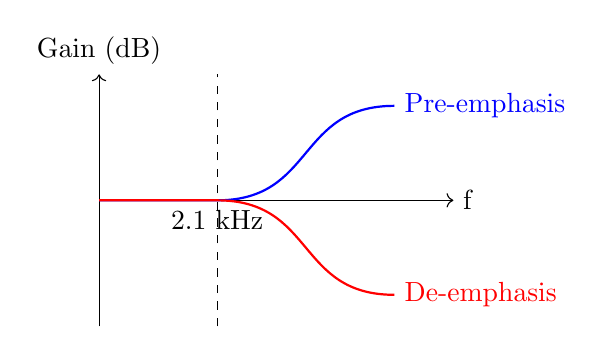
\begin{tikzpicture}[xscale=1.5, yscale=0.8]
        \draw[->] (0,0) -- (3,0) node[right] {f};
        \draw[->] (0,-2) -- (0,2) node[above] {Gain (dB)};
        \draw[blue, thick] (0,0) -- (1,0) to[out=0,in=180] (2.5,1.5) node[right] {Pre-emphasis};
        \draw[red, thick] (0,0) -- (1,0) to[out=0,in=180] (2.5,-1.5) node[right] {De-emphasis};
        \draw[dashed] (1,-2) -- (1,2);
        \node[below] at (1,0) {2.1 kHz};
    \end{tikzpicture}
    \captionof{figure}{Pre-emphasis and De-emphasis Frequency Response}
    \end{center}

    \begin{mnemonicbox}
    "HIGH-LOW" - HIGHer frequencies boosted at transmitter, LOWered at receiver
    \end{mnemonicbox}
\end{solutionbox}

\questionmarks{2}{c}{7}
\textbf{Compare narrowband FM and wideband FM.}

\begin{solutionbox}
    \textbf{Comparison of Narrowband FM and Wideband FM:}

    \begin{center}
    \begin{tabulary}{\linewidth}{L L L}
        \hline
        \textbf{Parameter} & \textbf{Narrowband FM} & \textbf{Wideband FM} \\
        \hline
        \textbf{Modulation Index ($\beta$)} & $\beta \ll 1$ (typically $<0.5$) & $\beta \gg 1$ (typically $>5$) \\
        \textbf{Bandwidth} & $2f_m$ (twice message bandwidth) & $2f_m(\beta+1)$ (Carson's rule) \\
        \textbf{Significant Sidebands} & Only first pair of sidebands & Multiple sidebands \\
        \textbf{Applications} & Mobile communication, two-way radio & FM broadcasting, high-fidelity audio \\
        \textbf{Signal Quality} & Lower fidelity, less noise immunity & Higher fidelity, better noise immunity \\
        \textbf{Power Efficiency} & Higher & Lower \\
        \textbf{Spectrum Utilization} & Efficient & Less efficient \\
        \textbf{Circuit Complexity} & Simpler & More complex \\
        \hline
    \end{tabulary}
    \end{center}

    \begin{center}
    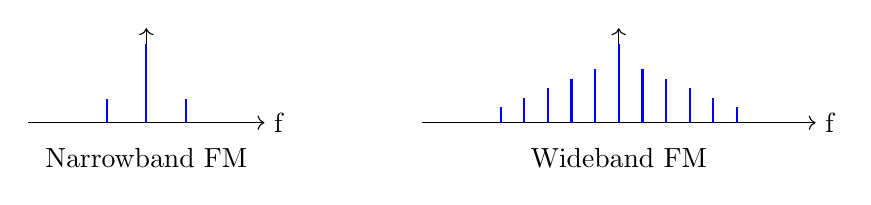
\begin{tikzpicture}
        % Narrowband
        \begin{scope}[xshift=-3cm]
            \draw[->] (-1.5,0) -- (1.5,0) node[right] {f};
            \draw[->] (0,0) -- (0,1.2);
            \draw[thick, blue] (0,0) -- (0,1);
            \draw[thick, blue] (-0.5,0) -- (-0.5,0.3);
            \draw[thick, blue] (0.5,0) -- (0.5,0.3);
            \node[below] at (0,-0.2) {Narrowband FM};
        \end{scope}
        
        % Wideband
        \begin{scope}[xshift=3cm]
            \draw[->] (-2.5,0) -- (2.5,0) node[right] {f};
            \draw[->] (0,0) -- (0,1.2);
            \draw[thick, blue] (0,0) -- (0,1);
             \foreach \x in {0.3, 0.6, 0.9, 1.2, 1.5} {
                \draw[thick, blue] (\x,0) -- (\x, {0.8-\x*0.4});
                \draw[thick, blue] (-\x,0) -- (-\x, {0.8-\x*0.4});
            }
            \node[below] at (0,-0.2) {Wideband FM};
        \end{scope}
    \end{tikzpicture}
    \captionof{figure}{Spectrum Comparison}
    \end{center}

    \begin{mnemonicbox}
    "BASPCB" - Bandwidth, Applications, Sidebands, Power, Complexity, Beta
    \end{mnemonicbox}
\end{solutionbox}

\questionmarks{3}{a}{3}
\textbf{Define any FOUR characteristics of radio receiver.}

\begin{solutionbox}
    \textbf{Characteristics of Radio Receiver:}

    \begin{enumerate}
        \item \textbf{Sensitivity:}
        \begin{itemize}
            \item Ability to amplify weak signals.
            \item Measured in microvolts ($\mu V$).
            \item Typically 1-10$\mu V$ for good receivers.
        \end{itemize}

        \item \textbf{Selectivity:}
        \begin{itemize}
            \item Ability to separate desired signal from adjacent channels.
            \item Determined by bandwidth of IF amplifier.
            \item Measured in dB at specific frequency offsets.
        \end{itemize}

        \item \textbf{Fidelity:}
        \begin{itemize}
            \item Accuracy in reproducing original signal.
            \item Depends on bandwidth and distortion.
            \item Measured as frequency response flatness.
        \end{itemize}

        \item \textbf{Image Frequency Rejection:}
        \begin{itemize}
            \item Ability to reject signals at image frequency ($f_i = f_s \pm 2f_{IF}$).
            \item Measured in dB.
            \item Higher values indicate better performance.
        \end{itemize}
    \end{enumerate}

    \begin{mnemonicbox}
    "SFID" - Sensitivity, Fidelity, Image rejection, selectivity Determines quality
    \end{mnemonicbox}
\end{solutionbox}

\questionmarks{3}{b}{4}
\textbf{Explain Diode Detector circuit.}

\begin{solutionbox}
    \textbf{Diode Detector Circuit:}

    \textbf{Purpose:}
    \begin{itemize}
        \item Extracts original message signal from AM wave.
        \item Also called envelope detector.
    \end{itemize}

    \textbf{Circuit components:}
    \begin{itemize}
        \item Diode: Rectifies AM signal.
        \item RC network: Filters carrier frequency.
        \item R \& C values: $RC \gg 1/f_c$ and $RC \ll 1/f_m$.
    \end{itemize}

    \textbf{Operation:}
    \begin{enumerate}
        \item Diode conducts during positive half-cycles.
        \item Capacitor charges to peak value.
        \item Capacitor discharges through resistor.
        \item RC time constant critical for proper demodulation.
    \end{enumerate}

    \begin{center}
    \begin{circuitikz}[font=\footnotesize]
        \draw (0,0) node[left]{AM Input} to[diode, l=D] (2,0) coordinate (top);
        \draw (top) to[C, l=C] (2,-1.5) coordinate (bot) node[ground]{};
        \draw (top) -- (3.5,0) coordinate (out) node[right]{Output};
        \draw (3.5,0) to[R, l=R] (3.5,-1.5) -- (bot);
        \draw (0,-1.5) node[left]{GND} -- (bot);
    \end{circuitikz}
    \captionof{figure}{Diode Detector}
    \end{center}

    \textbf{Waveforms:}
    \begin{center}
    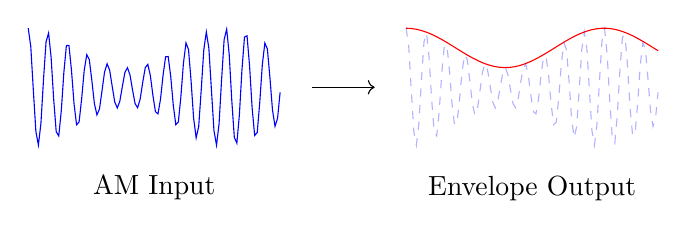
\begin{tikzpicture}[xscale=0.8, yscale=0.5]
        % AM Input
        \draw[blue] plot[domain=0:4, samples=100] (\x, {(1+0.5*cos(deg(2*\x)))*cos(deg(20*\x))});
        \node[below] at (2,-2) {AM Input};
        
        \draw[->] (4.5, 0) -- (5.5, 0);

        % Output
        \begin{scope}[xshift=6cm]
            \draw[red] plot[domain=0:4, samples=50] (\x, {1+0.5*cos(deg(2*\x))});
             \draw[blue, dashed, opacity=0.3] plot[domain=0:4, samples=100] (\x, {(1+0.5*cos(deg(2*\x)))*cos(deg(20*\x))});
             \node[below] at (2,-2) {Envelope Output};
        \end{scope}
    \end{tikzpicture}
    \end{center}

    \begin{mnemonicbox}
    "DRCO" - Diode Rectifies, Capacitor holds peaks, Output follows envelope
    \end{mnemonicbox}
\end{solutionbox}

\questionmarks{3}{c}{7}
\textbf{Draw and explain block diagram of super heterodyne receiver.}

\begin{solutionbox}
    \textbf{Super Heterodyne Receiver:}

    \textbf{Block Diagram:}
    
    \begin{center}
    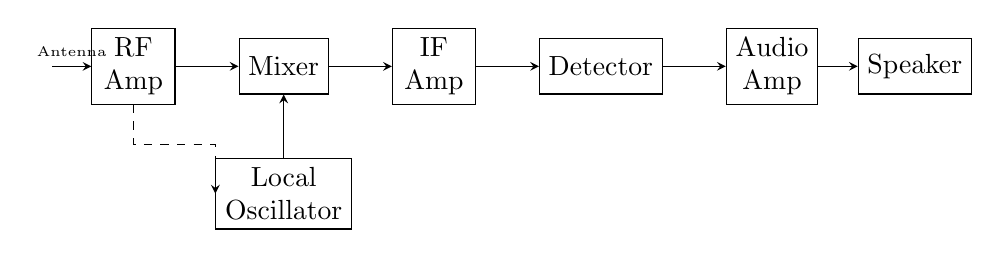
\begin{tikzpicture}[auto, node distance=1.5cm,
        block/.style={draw, rectangle, minimum height=2em, minimum width=3em, align=center, fill=white},
        input/.style={coordinate},
        output/.style={coordinate},
        >=stealth
    ]
        \node [input] (antenna) {};
        \node [block, right=0.5cm of antenna] (rf) {RF\\Amp};
        \node [block, right=0.8cm of rf] (mixer) {Mixer};
        \node [block, right=0.8cm of mixer] (if) {IF\\Amp};
        \node [block, right=0.8cm of if] (det) {Detector};
        \node [block, right=0.8cm of det] (audio) {Audio\\Amp};
        \node [block, right=0.5cm of audio] (spk) {Speaker};
        \node [block, below=0.8cm of mixer] (lo) {Local\\Oscillator};

        \draw [->] (antenna) -- node[above, font=\tiny]{Antenna} (rf);
        \draw [->] (rf) -- (mixer);
        \draw [->] (mixer) -- (if);
        \draw [->] (if) -- (det);
        \draw [->] (det) -- (audio);
        \draw [->] (audio) -- (spk);
        \draw [->] (lo) -- (mixer);
        \draw [->, dashed] (rf.south) -- +(0,-0.5) -| (lo.west); % Gang tuning

    \end{tikzpicture}
    \captionof{figure}{Superheterodyne Receiver Block Diagram}
    \end{center}

    \textbf{Function of each block:}
    \begin{enumerate}
        \item \textbf{RF Amplifier:} Amplifies weak RF signals, provides selectivity, improves SNR.
        \item \textbf{Local Oscillator:} Generates stable frequency $f_{LO} = f_{RF} + f_{IF}$ (high-side injection).
        \item \textbf{Mixer:} Combines RF with LO to produce IF ($f_{IF} = |f_{RF} - f_{LO}|$).
        \item \textbf{IF Amplifier:} Fixed frequency amplification (455kHz for AM), provides gain and selectivity.
        \item \textbf{Detector:} Demodulates IF signal to extract message.
        \item \textbf{Audio Amplifier:} Amplifies message for speaker.
    \end{enumerate}

    \textbf{Advantages:} Better selectivity/sensitivity, stable gain, reduced tracking problems.

    \begin{mnemonicbox}
    "RLMIDS" - RF amp, Local oscillator, Mixer, IF amp, Detector, Speaker
    \end{mnemonicbox}
\end{solutionbox}

% Part 2 Content

\questionmarks{3}{a}{3}
\textbf{Describe AGC principle and its application in Radio receiver.}

\begin{solutionbox}
    \textbf{AGC (Automatic Gain Control) Principle:}

    \textbf{Definition:}
    \begin{itemize}
        \item Circuit that automatically adjusts receiver gain based on signal strength.
        \item Maintains constant output level despite varying input signals.
    \end{itemize}

    \textbf{Working principle:}
    \begin{enumerate}
        \item Detects received signal strength.
        \item Generates control voltage proportional to signal.
        \item Applies negative feedback to reduce gain for strong signals.
        \item Increases gain for weak signals.
    \end{enumerate}

    \textbf{Application in Radio Receiver:}
    \begin{itemize}
        \item \textbf{Prevents overloading:} Protects against strong signal distortion.
        \item \textbf{Compensates fading:} Maintains constant volume during signal fading.
        \item \textbf{IF amplifier control:} Primarily applied to IF stages.
        \item \textbf{Improves dynamic range:} Handles wide range of signal strengths.
    \end{itemize}

    \begin{center}
    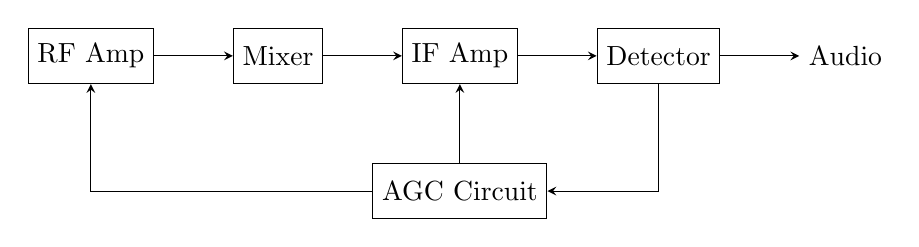
\begin{tikzpicture}[auto, node distance=1.5cm,
        block/.style={draw, rectangle, minimum height=2em, minimum width=3em, align=center},
        input/.style={coordinate},
        >=stealth
    ]
        \node [block] (rf) {RF Amp};
        \node [block, right=1cm of rf] (mixer) {Mixer};
        \node [block, right=1cm of mixer] (if) {IF Amp};
        \node [block, right=1cm of if] (det) {Detector};
        \node [coordinate, right=1cm of det] (out) {};
        \node [block, below=1cm of if] (agc) {AGC Circuit};

        \draw [->] (rf) -- (mixer);
        \draw [->] (mixer) -- (if);
        \draw [->] (if) -- (det);
        \draw [->] (det) -- (out) node[right] {Audio};
        
        \draw [->] (det.south) |- (agc.east);
        \draw [->] (agc.west) -| (rf.south);
        \draw [->] (agc.north) -- (if.south);

    \end{tikzpicture}
    \captionof{figure}{AGC in Superheterodyne Receiver}
    \end{center}

    \begin{mnemonicbox}
    "FADS" - Fading compensation, Automatic adjustment, Dynamic range, Signal consistency
    \end{mnemonicbox}
\end{solutionbox}

\questionmarks{3}{b}{4}
\textbf{Write short-note on intermediate frequency}

\begin{solutionbox}
    \textbf{Intermediate Frequency (IF):}

    \textbf{Definition:}
    \begin{itemize}
        \item Fixed frequency to which incoming RF signal is converted in superheterodyne receivers.
        \item Result of mixing (heterodyning) RF signal with local oscillator.
    \end{itemize}

    \textbf{Standard IF values:}
    \begin{itemize}
        \item \textbf{AM radio:} 455 kHz
        \item \textbf{FM radio:} 10.7 MHz
        \item \textbf{TV receivers:} 38-41 MHz
    \end{itemize}

    \textbf{Importance:}
    \begin{itemize}
        \item \textbf{Consistent gain:} Amplifiers operate at fixed frequency.
        \item \textbf{Better selectivity:} Narrowband filters at fixed frequency.
        \item \textbf{Simplified design:} Easier to design efficient fixed-frequency stages.
    \end{itemize}

    \textbf{Selection criteria:}
    \begin{itemize}
        \item High enough to provide good image rejection.
        \item Low enough for practical filter Q and gain.
        \item Should avoid harmonics of common signals.
    \end{itemize}

    \textbf{Image frequency calculation:}
    \begin{itemize}
        \item High-side injection: $f_{image} = f_{RF} + 2f_{IF}$
        \item Low-side injection: $f_{image} = f_{RF} - 2f_{IF}$
    \end{itemize}

    \begin{mnemonicbox}
    "CIGS" - Conversion, Improved selectivity, Gain stability, Simplified design
    \end{mnemonicbox}
\end{solutionbox}

\questionmarks{3}{c}{7}
\textbf{Explain phase discriminator circuit for FM detection.}

\begin{solutionbox}
    \textbf{Phase Discriminator for FM Detection:}

    \textbf{Purpose:}
    \begin{itemize}
        \item Converts frequency variations in FM signal to amplitude variations.
        \item Demodulates FM signal to recover original message.
    \end{itemize}

    \textbf{Working principle:}
    \begin{enumerate}
        \item Input FM signal splits into two paths.
        \item Reference path goes directly to center tap.
        \item Phase-shifted path passes through LC network.
        \item Phase shift varies with frequency deviation.
        \item Two diodes produce voltages proportional to phase difference.
        \item Output voltage varies with input frequency.
    \end{enumerate}

    \begin{center}
    \begin{circuitikz}[font=\footnotesize]
        % Transformers are hard in basic tikz, simplifying
        \draw (0,0) node[left] {FM Input} to[L] (0,-2);
        \draw (1,0) to[L] (1,-2);
        \draw (1,-1) -- (2,-1); % Center tap
        
        \draw (1,0) -- (2,0) to[diode, l=$D_1$] (4,0) coordinate (top);
        \draw (1,-2) -- (2,-2) to[diode, l=$D_2$] (4,-2) coordinate (bot);
        
        \draw (top) to[R, l=$R_1$] (4,-1) coordinate (mid);
        \draw (mid) to[R, l=$R_2$] (bot);
        \draw (mid) -- (5,-1) node[right] {Output};
        
        \draw (top) to[C, l=$C_1$] (3,-1) -- (mid);
        \draw (bot) to[C, l=$C_2$] (3,-1);
        
        \draw (2,-1) to[C, l=$C_c$] (0,0); % Coupling
    \end{circuitikz}
    \captionof{figure}{Foster-Seeley Discriminator}
    \end{center}

    \textbf{S-curve response:}
    \begin{center}
    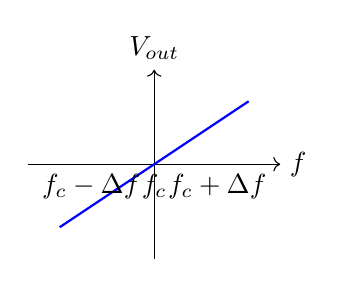
\begin{tikzpicture}[scale=0.8]
        \draw[->] (0,-1.5) -- (0,1.5) node[above] {$V_{out}$};
        \draw[->] (-2,0) -- (2,0) node[right] {$f$};
        \draw[thick, blue] (-1.5,-1) -- (1.5,1);
        \node[below] at (0,0) {$f_c$};
        \node[below] at (-1,0) {$f_c-\Delta f$};
        \node[below] at (1,0) {$f_c+\Delta f$};
    \end{tikzpicture}
    \captionof{figure}{Discriminator S-Curve}
    \end{center}

    \begin{mnemonicbox}
    "PSDO" - Phase shift Demodulates, Signal frequency determines Output
    \end{mnemonicbox}
\end{solutionbox}

\questionmarks{4}{a}{3}
\textbf{Compare analog and digital communication techniques}

\begin{solutionbox}
    \textbf{Comparison of Analog vs. Digital Communication:}

    \begin{center}
    \begin{tabulary}{\linewidth}{L L L}
        \hline
        \textbf{Parameter} & \textbf{Analog Communication} & \textbf{Digital Communication} \\
        \hline
        \textbf{Signal} & Continuous waveform & Discrete binary values \\
        \textbf{Bandwidth} & Less bandwidth required & More bandwidth required \\
        \textbf{Noise Immunity} & Poor, noise accumulates & Excellent, error correction possible \\
        \textbf{Power Efficiency} & Less efficient & More efficient \\
        \textbf{Quality} & Degrades with distance & Maintains quality until SNR threshold \\
        \textbf{Multiplexing} & FDM primarily used & TDM primarily used \\
        \textbf{System Complexity} & Simpler & More complex \\
        \textbf{Cost} & Lower & Higher but decreasing \\
        \hline
    \end{tabulary}
    \end{center}

    \begin{mnemonicbox}
    "BNPQ MCE" - Bandwidth, Noise immunity, Power, Quality, Multiplexing, Complexity, Efficiency
    \end{mnemonicbox}
\end{solutionbox}

\questionmarks{4}{b}{4}
\textbf{Explain Adaptive delta modulation with its application.}

\begin{solutionbox}
    \textbf{Adaptive Delta Modulation (ADM):}

    \textbf{Working principle:}
    \begin{itemize}
        \item Improved version of Delta Modulation (DM).
        \item Uses variable step size adjusted to signal slope.
        \item Increases step size for rapid changes (prevents slope overload).
        \item Decreases step size for slow changes (prevents granular noise).
    \end{itemize}

    \textbf{Block Diagram:}
    \begin{center}
    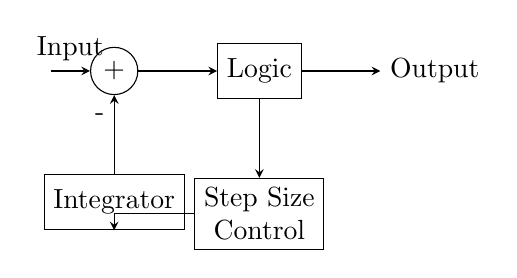
\begin{tikzpicture}[auto, node distance=1.5cm,
        block/.style={draw, rectangle, minimum height=2em, minimum width=3em, align=center},
        sum/.style={draw, circle, inner sep=0pt, minimum size=6mm},
        >=stealth
    ]
        \node [coordinate] (input) {};
        \node [sum, right=0.5cm of input] (sum) {+};
        \node [block, right=1cm of sum] (logic) {Logic};
        \node [block, below=1cm of logic] (step) {Step Size\\Control};
        \node [block, below=1cm of sum] (int) {Integrator};
        \node [coordinate, right=1cm of logic] (output) {};

        \draw [->] (input) -- node[above]{Input} (sum);
        \draw [->] (sum) -- (logic);
        \draw [->] (logic) -- (output) node[right]{Output};
        \draw [->] (logic.south) -- (step.north);
        \draw [->] (step.west) -| (int.south);
        \draw [->] (int.north) -- (sum.south) node[near end, left] {-};

    \end{tikzpicture}
    \captionof{figure}{Adaptive Delta Modulation}
    \end{center}

    \textbf{Applications:}
    \begin{itemize}
        \item Speech transmission.
        \item Audio compression.
        \item Telemetry systems.
        \item Military communications.
    \end{itemize}

    \begin{mnemonicbox}
    "VSOG" - Variable Step size Overcomes Granular noise \& slope overload
    \end{mnemonicbox}
\end{solutionbox}

\questionmarks{4}{c}{7}
\textbf{Draw \& explain block diagram of PCM system.}

\begin{solutionbox}
    \textbf{Pulse Code Modulation (PCM) System:}

    \textbf{Block Diagram:}

    \begin{center}
    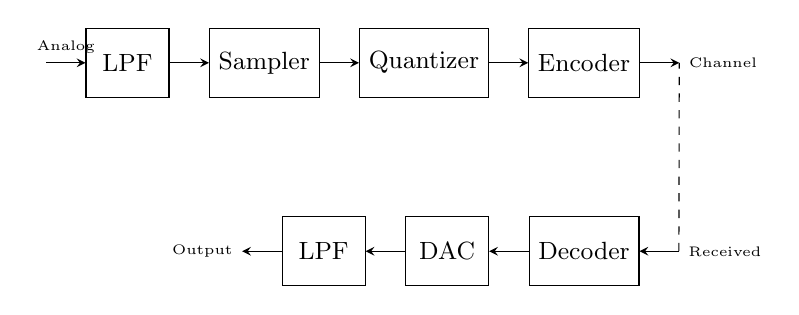
\begin{tikzpicture}[auto, node distance=1.2cm,
        block/.style={draw, rectangle, minimum height=2.5em, minimum width=3em, align=center, font=\small},
        >=stealth
    ]
        % Transmitter
        \node [coordinate] (input) {};
        \node [block, right=0.5cm of input] (lpf) {LPF};
        \node [block, right=0.5cm of lpf] (sampler) {Sampler};
        \node [block, right=0.5cm of sampler] (quant) {Quantizer};
        \node [block, right=0.5cm of quant] (enc) {Encoder};
        \node [coordinate, right=0.5cm of enc] (txout) {};
        
        \draw [->] (input) -- node[above, font=\tiny]{Analog} (lpf);
        \draw [->] (lpf) -- (sampler);
        \draw [->] (sampler) -- (quant);
        \draw [->] (quant) -- (enc);
        \draw [->] (enc) -- (txout) node[right, font=\tiny]{Channel};

        % Receiver
        \node [block, below=1.5cm of enc] (dec) {Decoder};
        \node [coordinate, right=0.5cm of dec] (rxin) {};
        \node [block, left=0.5cm of dec] (dac) {DAC};
        \node [block, left=0.5cm of dac] (lpf2) {LPF};
        \node [coordinate, left=0.5cm of lpf2] (output) {};
        
        \draw [<-] (dec) -- (rxin) node[right, font=\tiny]{Received};
        \draw [->] (dec) -- (dac);
        \draw [->] (dac) -- (lpf2);
        \draw [->] (lpf2) -- (output) node[left, font=\tiny]{Output};

        \draw[dashed] (rxin) -- (txout);
    \end{tikzpicture}
    \captionof{figure}{PCM System Block Diagram}
    \end{center}

    \textbf{Transmitter components:}
    \begin{enumerate}
        \item \textbf{Sample \& Hold:} Samples analog signal at Nyquist rate ($f_s \ge 2f_{max}$).
        \item \textbf{Quantizer:} Divides amplitude into discrete levels, maps samples to nearest level.
        \item \textbf{Encoder:} Converts quantized levels to binary code.
    \end{enumerate}

    \textbf{Receiver components:}
    \begin{enumerate}
        \item \textbf{Decoder:} Converts binary to quantized levels.
        \item \textbf{DAC:} Produces staircase approximation.
        \item \textbf{Low-Pass Filter:} Smooths output, reconstructs original waveform.
    \end{enumerate}

    \begin{mnemonicbox}
    "SQEC-DFL" - Sample, Quantize, Encode, Channel - Decode, Filter, Listen
    \end{mnemonicbox}
\end{solutionbox}

\questionmarks{4}{a}{3}
\textbf{Explain quantization process and its necessity.}

\begin{solutionbox}
    \textbf{Quantization Process and its Necessity:}

    \textbf{Definition:} Process of mapping continuous amplitude values to discrete levels.

    \textbf{Types:}
    \begin{itemize}
        \item \textbf{Uniform quantization:} Equal step size.
        \item \textbf{Non-uniform quantization:} Variable step size.
    \end{itemize}

    \textbf{Necessity:}
    \begin{itemize}
        \item \textbf{Digital representation:} Enables conversion to binary.
        \item \textbf{Storage efficiency:} Allows finite storage.
        \item \textbf{Processing capability:} Enables DSP.
        \item \textbf{Transmission benefits:} Error correction/encryption.
    \end{itemize}

    \textbf{Quantization error:} Max error = $\pm Q/2$ ($Q=$ step size). $SQNR = 6.02n + 1.76$ dB.

    \begin{center}
    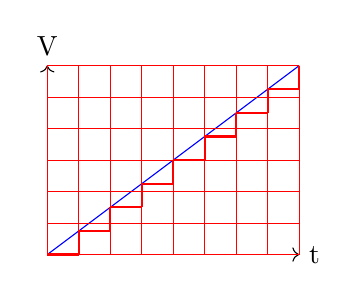
\begin{tikzpicture}[scale=0.8]
        \draw[->] (0,0) -- (4,0) node[right] {t};
        \draw[->] (0,0) -- (0,3) node[above] {V};
        \draw[blue] (0,0) -- (4,3);
        \draw[red, step=0.5] (0,0) grid (4,3);
        \foreach \x in {0,0.5,...,3.5} {
            \draw[thick, red] (\x, {0.75*\x}) -- (\x+0.5, {0.75*\x});
            \draw[thick, red] (\x+0.5, {0.75*\x}) -- (\x+0.5, {0.75*(\x+0.5)});
        }
    \end{tikzpicture}
    \captionof{figure}{Quantization Staircase}
    \end{center}

    \begin{mnemonicbox}
    "DEBS" - Digitization Enables Binary Storage
    \end{mnemonicbox}
\end{solutionbox}

\questionmarks{4}{b}{4}
\textbf{Explain PCM receiver.}

\begin{solutionbox}
    \textbf{PCM Receiver:}

    \begin{center}
    
\begin{tikzpicture}[auto, node distance=1.5cm,
        block/.style={draw, rectangle, minimum height=2em, minimum width=3em, align=center},
        >=stealth
    ]
        \node [block] (buf) {Buffer};
        \node [block, right=1cm of buf] (dec) {Decoder};
        \node [block, right=1cm of dec] (dac) {DAC};
        \node [block, right=1cm of dac] (lpf) {Low Pass\\Filter};
        \node [coordinate, left=1cm of buf] (in) {};
        \node [coordinate, right=1cm of lpf] (out) {};

        \draw [->] (in) -- node[above]{PCM Input} (buf);
        \draw [->] (buf) -- (dec);
        \draw [->] (dec) -- (dac);
        \draw [->] (dac) -- (lpf);
        \draw [->] (lpf) -- (out) node[right]{Analog Output};
    \end{tikzpicture}
    \captionof{figure}{PCM Receiver}
    \end{center}

    \textbf{Components:}
    \begin{itemize}
        \item \textbf{Buffer:} Stores data, reduces jitter.
        \item \textbf{Decoder:} Converts binary to quantized levels.
        \item \textbf{DAC:} Creates staircase waveform.
        \item \textbf{Low-Pass Filter:} Smooths waveform.
    \end{itemize}

    \begin{mnemonicbox}
    "BDFL" - Buffer stores, Decoder converts, Filter smooths, Listen to output
    \end{mnemonicbox}
\end{solutionbox}

\questionmarks{4}{c}{7}
\textbf{What is sampling? Explain types of sampling in brief.}

\begin{solutionbox}
    \textbf{Sampling:} Process of converting continuous-time signal into discrete-time signal.

    \textbf{Nyquist Theorem:} $f_s \ge 2f_{max}$ to prevent aliasing.

    \textbf{Types of Sampling:}
    \begin{itemize}
        \item \textbf{Ideal Sampling:} Instantaneous impulses (theoretical).
        \item \textbf{Natural Sampling:} Pulses follow signal shape.
        \item \textbf{Flat-Top Sampling:} Sample-and-hold (staircase).
    \end{itemize}

    \begin{center}
    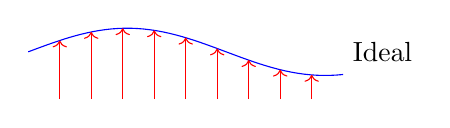
\begin{tikzpicture}[xscale=0.8, yscale=0.6]
        % Signal
        \draw[blue] plot[domain=0:5, samples=50] (\x, {1+0.5*sin(deg(\x))});
        
        % Ideal
        \foreach \x in {0.5, 1.0, ..., 4.5} {
            \draw[->, red] (\x, 0) -- (\x, {1+0.5*sin(deg(\x))});
        }
        \node[right] at (5,1) {Ideal};
    \end{tikzpicture}
    \quad
    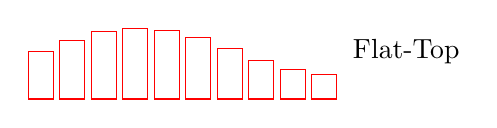
\begin{tikzpicture}[xscale=0.8, yscale=0.6]
        % Flat Top
        \foreach \x in {0, 0.5, ..., 4.5} {
            \draw[red] (\x, 0) rectangle (\x+0.4, {1+0.5*sin(deg(\x))});
        }
        \node[right] at (5,1) {Flat-Top};
    \end{tikzpicture}
    \captionof{figure}{Sampling Types}
    \end{center}

    \begin{mnemonicbox}
    "INF" - Ideal (impulses), Natural (pulse-shaped), Flat-top (staircase)
    \end{mnemonicbox}
\end{solutionbox}

\questionmarks{5}{a}{3}
\textbf{List the need of Multiplexing.}

\begin{solutionbox}
    \textbf{Need for Multiplexing:}

    \begin{itemize}
        \item \textbf{Bandwidth Utilization}: Efficient use of medium.
        \item \textbf{Cost Reduction}: Shares expensive medium.
        \item \textbf{Infrastructure Optimization}: Fewer wires/connections.
        \item \textbf{Spectrum Efficiency}: Maximizes frequency use.
        \item \textbf{Network Capacity}: More users/channels.
        \item \textbf{Flexibility}: Dynamic resource allocation.
    \end{itemize}

    \begin{mnemonicbox}
    "BCSINF" - Bandwidth, Cost, Spectrum, Infrastructure, Network capacity, Flexibility
    \end{mnemonicbox}
\end{solutionbox}

\questionmarks{5}{b}{4}
\textbf{Explain working of DPCM.}

\begin{solutionbox}
    \textbf{Differential Pulse Code Modulation (DPCM):}

    \begin{itemize}
        \item Encodes difference between current and predicted sample.
        \item Reduces bit rate by exploiting signal correlation.
    \end{itemize}

    \begin{center}
    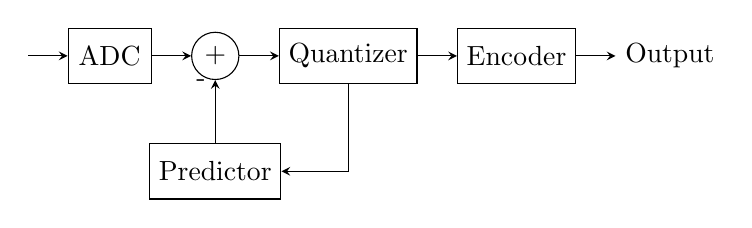
\begin{tikzpicture}[auto, node distance=1.5cm,
        block/.style={draw, rectangle, minimum height=2em, minimum width=3em, align=center},
        sum/.style={draw, circle, inner sep=0pt, minimum size=6mm},
        >=stealth
    ]
        \node [coordinate] (in) {};
        \node [block, right=0.5cm of in] (adc) {ADC};
        \node [sum, right=0.5cm of adc] (sum) {+};
        \node [block, right=0.5cm of sum] (quant) {Quantizer};
        \node [block, right=0.5cm of quant] (enc) {Encoder};
        \node [coordinate, right=0.5cm of enc] (out) {};
        \node [block, below=0.8cm of sum] (pred) {Predictor};

        \draw [->] (in) -- (adc);
        \draw [->] (adc) -- (sum);
        \draw [->] (sum) -- (quant);
        \draw [->] (quant) -- (enc);
        \draw [->] (enc) -- (out) node[right]{Output};
        \draw [->] (quant.south) |- (pred.east);
        \draw [->] (pred.north) -- (sum.south) node[left]{-};
    \end{tikzpicture}
    \captionof{figure}{DPCM Transmitter}
    \end{center}

    \begin{mnemonicbox}
    "PDQE" - Predict sample, Difference calculated, Quantize error, Encode result
    \end{mnemonicbox}
\end{solutionbox}

\questionmarks{5}{c}{7}
\textbf{The binary data 1011001 is to be transmitted using following line coding techniques: (i) Unipolar RZ and NRZ (ii) Polar RZ and NRZ (iii) AMI (iv) Manchester. Draw all the waveforms.}

\begin{solutionbox}
    \textbf{Line Coding of Binary Data: 1011001}

    \begin{center}
    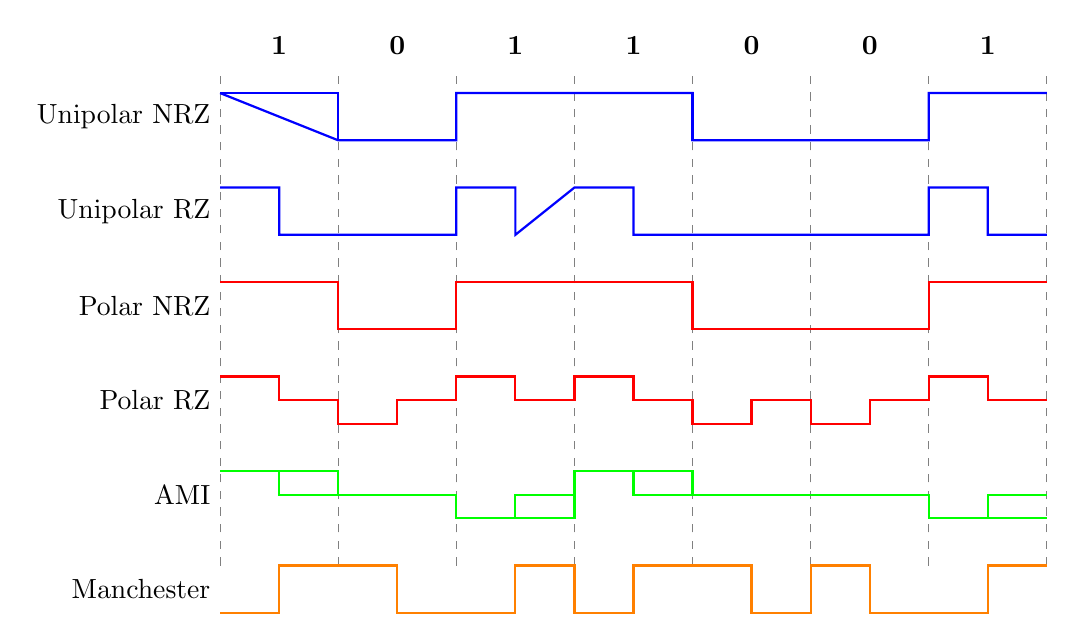
\begin{tikzpicture}[xscale=1.5, yscale=0.6]
        \foreach \x/\b in {0/1, 1/0, 2/1, 3/1, 4/0, 5/0, 6/1} {
            \node at (\x+0.5, 9) {\textbf{\b}};
            \draw[dashed, gray] (\x, -2) -- (\x, 8.5);
            \draw[dashed, gray] (\x+1, -2) -- (\x+1, 8.5);
        }
        
        \node[left] at (0, 7.5) {Unipolar NRZ};
        \draw[thick, blue] (0,8) -- (1,7) -- (2,7) -- (2,8) -- (4,8) -- (4,7) -- (6,7) -- (6,8) -- (7,8); 
        % Wait, Uni NRZ: 1=High, 0=Low.
        % 1: High (0-1)
        % 0: Low (1-2)
        % 1: High (2-3)
        % 1: High (3-4)
        % 0: Low (4-5)
        % 0: Low (5-6)
        % 1: High (6-7)
        \draw[thick, blue] (0,8) -- (1,8) -- (1,7) -- (2,7) -- (2,8) -- (4,8) -- (4,7) -- (6,7) -- (6,8) -- (7,8);

        \node[left] at (0, 5.5) {Unipolar RZ};
        % 1: High half, Low half
        % 0: Low full
        \draw[thick, blue] (0,6) -- (0.5,6) -- (0.5,5) -- (2,5) -- (2,6) -- (2.5,6) -- (2.5,5) -- (3,6) -- (3.5,6) -- (3.5,5) -- (6,5) -- (6,6) -- (6.5,6) -- (6.5,5) -- (7,5);

        \node[left] at (0, 3.5) {Polar NRZ};
        % 1: +V
        % 0: -V
        \draw[thick, red] (0,4) -- (1,4) -- (1,3) -- (2,3) -- (2,4) -- (4,4) -- (4,3) -- (6,3) -- (6,4) -- (7,4);

        \node[left] at (0, 1.5) {Polar RZ};
        % 1: +V half, 0 half
        % 0: -V half, 0 half
        \draw[thick, red] (0,2) -- (0.5,2) -- (0.5,1.5) -- (1,1.5) -- (1,1) -- (1.5,1) -- (1.5,1.5) -- (2,1.5) -- (2,2) -- (2.5,2) -- (2.5,1.5) -- (3,1.5) -- (3,2) -- (3.5,2) -- (3.5,1.5) -- (4,1.5) -- (4,1) -- (4.5,1) -- (4.5,1.5) -- (5,1.5) -- (5,1) -- (5.5,1) -- (5.5,1.5) -- (6,1.5) -- (6,2) -- (6.5,2) -- (6.5,1.5) -- (7,1.5);
        
        \node[left] at (0, -0.5) {AMI};
        % 1: Alt +V/-V
        % 0: 0V
        % 1(+), 0(0), 1(-), 1(+), 0(0), 0(0), 1(-)
        \draw[thick, green] (0,0) -- (1,0) -- (1,-0.5) -- (2,-0.5) -- (2,-1) -- (3,-1) -- (3,0) -- (4,0) -- (4,-0.5) -- (6,-0.5) -- (6,-1) -- (7,-1);
        % Wait, AMI usually RZ or NRZ? Usually RZ convention in problem solving unless specified. Let's assume AMI is RZ (standard).
         \draw[thick, green] (0,0) -- (0.5,0) -- (0.5,-0.5) -- (1,-0.5) -- (2,-0.5) -- (2,-1) -- (2.5,-1) -- (2.5,-0.5) -- (3,-0.5) -- (3,0) -- (3.5,0) -- (3.5,-0.5) -- (6,-0.5) -- (6,-1) -- (6.5,-1) -- (6.5,-0.5) -- (7,-0.5);

        \node[left] at (0, -2.5) {Manchester};
        % 1: Low->High
        % 0: High->Low
        \draw[thick, orange] (0,-3) -- (0.5,-3) -- (0.5,-2) -- (1,-2) -- (1,-2) -- (1.5,-2) -- (1.5,-3) -- (2,-3) -- (2,-3) -- (2.5,-3) -- (2.5,-2) -- (3,-2) -- (3,-3) -- (3.5,-3) -- (3.5,-2) -- (4,-2) -- (4,-2) -- (4.5,-2) -- (4.5,-3) -- (5,-3) -- (5,-2) -- (5.5,-2) -- (5.5,-3) -- (6,-3) -- (6,-3) -- (6.5,-3) -- (6.5,-2) -- (7,-2);
    \end{tikzpicture}
    \captionof{figure}{Line Coding Waveforms}
    \end{center}

    \begin{mnemonicbox}
    "UPRMA" - Unipolar, Polar, Return-to-zero, Manchester, AMI
    \end{mnemonicbox}
\end{solutionbox}

\questionmarks{5}{a}{3}
\textbf{Explain polar RZ and NRZ format}

\begin{solutionbox}
    \textbf{Polar RZ and NRZ Line Coding:}

    \textbf{Polar NRZ:}
    \begin{itemize}
        \item Binary 1: $+V$, Binary 0: $-V$
        \item No return to zero.
        \item Simple but poor clock recovery.
    \end{itemize}

    \textbf{Polar RZ:}
    \begin{itemize}
        \item Binary 1: $+V$ for half bit, 0 for rest.
        \item Binary 0: $-V$ for half bit, 0 for rest.
        \item Self-clocking, requires more bandwidth.
    \end{itemize}

    \begin{mnemonicbox}
    "HZRT" - Half bit active + Zero Return in RZ, full Time in NRZ
    \end{mnemonicbox}
\end{solutionbox}

\questionmarks{5}{b}{4}
\textbf{Explain delta modulation in brief.}

\begin{solutionbox}
    \textbf{Delta Modulation (DM):}

    \begin{itemize}
        \item Simplest differential encoding.
        \item 1 bit per sample (tracks slope).
        \item Susceptible to slope overload and granular noise.
    \end{itemize}

    \begin{center}
    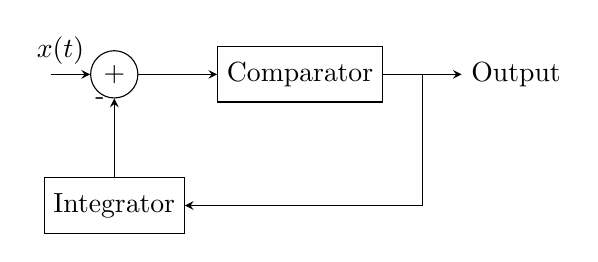
\begin{tikzpicture}[auto, node distance=1.5cm,
        block/.style={draw, rectangle, minimum height=2em, minimum width=3em, align=center},
        sum/.style={draw, circle, inner sep=0pt, minimum size=6mm},
        >=stealth
    ]
        \node [coordinate] (in) {};
        \node [sum, right=0.5cm of in] (sum) {+};
        \node [block, right=1cm of sum] (comp) {Comparator};
        \node [coordinate, right=1cm of comp] (out) {};
        \node [block, below=1cm of sum] (int) {Integrator};

        \draw [->] (in) -- (sum) node[near start, above] {$x(t)$};
        \draw [->] (sum) -- (comp);
        \draw [->] (comp) -- (out) node[right] {Output};
        \draw [->] (comp.east) -- ++(0.5,0) |- (int.east);
        \draw [->] (int.north) -- (sum.south) node[left] {-};
    \end{tikzpicture}
    \captionof{figure}{Delta Modulator}
    \end{center}

    \begin{mnemonicbox}
    "1BSG" - 1 Bit per Sample, Slope overload and Granular noise limitations
    \end{mnemonicbox}
\end{solutionbox}

\questionmarks{5}{c}{7}
\textbf{Explain PCM-TDM system.}

\begin{solutionbox}
    \textbf{PCM-TDM System:}

    \begin{itemize}
        \item Combines PCM (Analog to Digital) with TDM (Multiplexing).
        \item Multiple analog channels $\to$ PCM $\to$ Time Multiplexed.
    \end{itemize}

    \begin{center}
    \begin{tikzpicture}[auto, node distance=1cm,
        block/.style={draw, rectangle, minimum height=2em, minimum width=3em, align=center},
        mux/.style={draw, trapezium, trapezium angle=60, shape border rotate=270, minimum height=3em, align=center},
        >=stealth
    ]
        \node [block] (pcm1) {PCM 1};
        \node [block, below=0.5cm of pcm1] (pcm2) {PCM 2};
        \node [below=0.5cm of pcm2] (dots) {\vdots};
        \node [block, below=0.5cm of dots] (pcmn) {PCM N};

        \node [mux, right=1.5cm of pcm2, minimum height=4cm] (mux) {MUX};
        \node [block, right=1cm of mux] (frame) {Frame\\Format};
        \node [coordinate, right=1cm of frame] (out) {};

        \draw [->] (pcm1) -- (mux.west |- pcm1.east);
        \draw [->] (pcm2) -- (mux.west |- pcm2.east);
        \draw [->] (pcmn) -- (mux.west |- pcmn.east);
        \draw [->] (mux) -- (frame);
        \draw [->] (frame) -- (out) node[right] {PCM-TDM Out};

        \node [left=0.5cm of pcm1] {Ch 1};
        \node [left=0.5cm of pcm2] {Ch 2};
        \node [left=0.5cm of pcmn] {Ch N};
    \end{tikzpicture}
    \captionof{figure}{PCM-TDM System}
    \end{center}

    \textbf{TDM Frame:}
    \begin{center}
    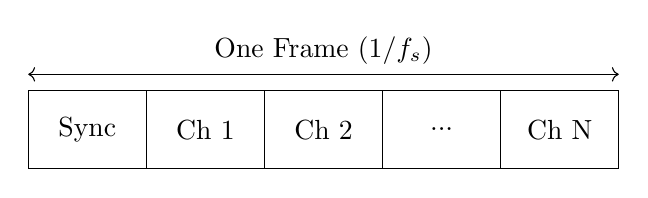
\begin{tikzpicture}
        \draw (0,0) rectangle (1.5,1) node[midway] {Sync};
        \draw (1.5,0) rectangle (3,1) node[midway] {Ch 1};
        \draw (3,0) rectangle (4.5,1) node[midway] {Ch 2};
        \draw (4.5,0) rectangle (6,1) node[midway] {...};
        \draw (6,0) rectangle (7.5,1) node[midway] {Ch N};
        \draw[<->] (0,1.2) -- (7.5,1.2) node[midway, above] {One Frame ($1/f_s$)};
    \end{tikzpicture}
    \end{center}

    \begin{mnemonicbox}
    "MSQT" - Multiplex, Sample, Quantize, Transmit
    \end{mnemonicbox}
\end{solutionbox}

\end{document}
